\documentclass[
  paper=192mm:108mm,
  fontsize=11pt,
  pagesize,
  parskip=half-,
  numbers=noendperiod,
  captions=nooneline
]{scrartcl}

\linespread{1.12}

\usepackage[T1]{fontenc}
% \usepackage{lmodern}
\usepackage[british]{babel}
\usepackage{microtype}
\usepackage{xcolor}
\usepackage{calc}
\usepackage[includeheadfoot,top=3.5mm,bottom=3.5mm,left=5.5mm,right=5.5mm,headsep=6.5mm,footskip=8.5mm]{geometry}
\usepackage{scrpage2}
\usepackage{titlesec}
\usepackage{tocstyle}

% \usepackage{bm}
\usepackage{tikz}
\usetikzlibrary{positioning}

\usepackage[notext,lcgreekalpha]{stix}
\usepackage{amsmath}
\usepackage{amsfonts}
\usepackage{mathtools}
\usepackage{xfrac}
\usepackage{relsize}

\renewcommand{\familydefault}{\sfdefault}

% page  style
\pagestyle{scrheadings}% activates  pagestyle  from  scrpage2
\clearscrheadfoot% clear  head  and  foot
\setkomafont{pageheadfoot}{\normalfont\color{white}\sffamily}% setting  for  page  head  and  foot
% optical  vertical  centering  of page  contents
\makeatletter
\renewcommand*{\@textbottom}{\vskip \z@ \@plus 1fil}
\newcommand*{\@texttop}{\vskip \z@ \@plus .5fil}
\addtolength{\parskip}{\z@\@plus .25fil}% stretch  parskip
\makeatother

\titlespacing{\section}{0mm}{0mm}{0mm}
\titlespacing{\subsection}{0mm}{0mm}{-1mm}
\titlespacing{\subsubsection}{0mm}{0mm}{-2mm}

\definecolor{mybgcolor}{HTML}{0E3655}
\newcommand*{\runninghead}{Outline}
\newcommand*{\myauthor}{Rupert Horlick}
\newcommand*{\myuni}{University of Cambridge}

\ihead{% head  left
  \hspace{-2mm}%
  \begin{tikzpicture}[remember  picture,overlay]
    \node [xshift=\paperwidth/2,yshift=-\headheight] (mybar) at (current page.north west)[rectangle,fill,inner sep=0pt,minimum width=\paperwidth,minimum height=2\headheight,top color=mybgcolor!64,bottom color=mybgcolor]{};% bar
    \node[below of=mybar,yshift=3.3mm,rectangle,shade,inner sep=0pt,minimum width=192mm,minimum height=1.5mm,top color=black!50,bottom color=white]{};% shadow
  \end{tikzpicture}%
  \runninghead
}

% \newlength{\footheight}
\setlength{\footheight}{8mm}
\addtokomafont{pagefoot}{\footnotesize}% size  for  foot
\setkomafont{pagenumber}{\color{white}}% white  page  number
\ifoot{% foot  left
  \hspace{-2mm}%
  \begin{tikzpicture}[remember picture,overlay]
    \node [xshift=\paperwidth/2,yshift=\footheight/2] at (current page.south west)[rectangle,fill,inner sep=0pt,minimum width=\paperwidth,minimum height=\footheight,top color=mybgcolor!64,bottom color=mybgcolor]{};% bar
  \end{tikzpicture}%
  \myauthor\ \raisebox{0.2mm}{$\vert$}\ \myuni
}
\ofoot[\pagemark\hspace{-2mm}]{\pagemark\hspace{-2mm}}% foot  right (plain  pages do also  have  page  numbers)

\AtBeginDocument{\renewcaptionname{british}{\contentsname}{}} %{\large Outline}}% change  name of toc
\makeatletter
\newtocstyle[noonewithdot]{nodotnopagenumber}{% define tocstyle  without  dots  and  page  numbers
  \settocfeature{pagenumberbox}{\@gobble}%
}
\makeatother
\usetocstyle{nodotnopagenumber}

\newcommand*{\sectionpage}[1]{
    \thispagestyle{empty}
    \begin{tikzpicture}[remember picture,overlay]
      \node[xshift=\paperwidth/2,yshift=-\paperheight/2] at (current page.north west) [rectangle,fill,inner sep=0pt,minimum width=\paperwidth,minimum height=\paperheight,top color=mybgcolor!64,bottom color=mybgcolor,text width=180mm,align=center,color=white] {\sffamily\huge #1};
    \end{tikzpicture}
    \clearpage
}

\usepackage{xparse}
%
\DeclareDocumentCommand\sectiona{s o m}{%
    \clearpage%
    \IfBooleanTF{#1}{%
        \renewcommand{\runninghead}{#3}%
    }{%
        \refstepcounter{section}%JB: Please don't aske mw, %
%why i am doing this, as they aren't printed anyway%
        \renewcommand{\runninghead}{#3}%always use the%
%       mandatory argument for the runninghead%
        \IfNoValueTF{#2}{%
            \addsectiontocentry{}{#3}%
            \sectionpage{#3}%
        }{%
            \addsectiontocentry{}{#2}%
            \sectionpage{#2}%
        }%
    }%
}%
\newcommand\subsectiona[1]{%
    \clearpage%
    \refstepcounter{subsection}%
    \renewcommand{\runninghead}{\small #1\par}%
    \addsubsectiontocentry{}{#1}%
}%
%

\makeatletter
\renewcommand\tableofcontents{%
    \@starttoc{toc}%
}
\makeatother

%%%%%%%%%%%%%%%%%%%%%%%%%%%%%%%%%%%%%%%%%%%%%%%%%%%%%%%%%%%%%%%%%%%%%%%%%%%%%%%%

\newcommand*{\cat}[1]{\mathbb{#1}}
\renewcommand{\circ}{\vysmwhtcircle}
\newcommand*{\Obj}{\mathsf{Obj}\,}
\newcommand*{\id}[1]{\mathsf{id}_{#1}}
\newcommand*{\SM}{\mathsf{SM}}
\newcommand*{\Fin}{\mathsf{Fin}}
\newcommand*{\List}{\mathsf{List}}
\newcommand*{\ListPerm}{\mathsf{ListPerm}}
\newcommand{\defeq}{\vcentcolon\equiv}
\newcommand{\spec}[2]{#1 \rightwavearrow #2}
\newcommand{\Quot}{\operatorname{Quot}_C(R)}
\newcommand{\q}{\operatorname{q}}
\newcommand{\rel}{\operatorname{rel}}

\begin{document}

\thispagestyle{empty}

\begin{tikzpicture}[remember picture,overlay]
  \node [xshift=\paperwidth/2,yshift=-\paperheight/2] at (current page.north west) [rectangle,fill,inner sep=0pt,minimum width=\paperwidth,minimum height=\paperheight,top color=mybgcolor!64,bottom color=mybgcolor,text width=180mm,align=center,color=white] {\sffamily\Huge Generalised Species of Structures \\ in Homotopy Type Theory Using Agda \\ \vspace{10mm} \Large \today};
\end{tikzpicture}

\clearpage

\tableofcontents

\sectiona{Introduction}

This project sits at the center of three main topics

\begin{center}
\begin{tikzpicture}[node distance=4cm and 0.6cm]
  \node (1) {Combinatorial Species};
  \node (2) [below left=of 1,text width=3cm,align=center] {Type Theory (HoTT/Agda)}
    edge[-] (1);
  \node (3) [below right=of 1,text width=4.5cm,align=center] {Categorical Models of Differential Linear Logic}
    edge[-] (1)
    edge[-] (2);
  \node (4) [below=2.3cm of 1] {$\cdot$};
\end{tikzpicture}
\end{center}

\sectiona{Combinatorial Species}

A combinatorial species consists of a rule, $F$, that associates

\begin{itemize}
  \item with every finite set, $U$, a finite set, $F[U]$
  \item with every bijection, $\sigma : U \to V$, a bijection, $F[\sigma] : F[U] \to F[V]$
\end{itemize}

and satisifies

\begin{itemize}
  \item $F[\id{U}] = \id{F[U]}$
  \item $F[\tau \circ \sigma] = F[\tau] \circ F[\sigma]$
\end{itemize}

\subsectiona{Sorted Species}

A $k$-sorted species, $F$, acts on finite multisets, associating
\begin{itemize}
  \item with every finite multiset, $U = (U_1,\dots,U_k)$, a finite set, $F[U_1,\dots,U_k]$
  \item with every bijective multifunction, $$\sigma : (U_1,\dots,U_k) \to (V_1,\dots,V_k),$$ a bijection, $$F[\sigma] : F[U_1,\dots,U_k] \to F[V_1,\dots,V_k]$$
\end{itemize}
Again this satisifies functoriality conditions

\subsectiona{$\SM$ Construction}

This notion of sorted species is linked to relational models of linear logic

Here we have operations on relations as the connectives of linear logic
\begin{align*}
  A \otimes B &\defeq A \times B & A \& B &\defeq A \uplus B \\
   I &\defeq \{\star\} & 1 &\defeq \varnothing
\end{align*}
$$A \multimap B \defeq A \otimes B$$

The exponential modality of linear logic is modelled by $\SM$, the finite-multiset construction
\begin{itemize}
  \item $\SM\,A \defeq \mathcal{M}_{fin}(A)$
  \item $\SM\,f \defeq \{([a_1,\dots,a_n],[b_1,\dots,b_n])\,|\,\forall i. (a_i,b_i) \in f\}$
\end{itemize}

\subsectiona{Generalised Species}

We can generalise the notion of relation between categories $\cat{C}$ and $\cat{D}$ as
$$\cat{C} \to \cat{D} \to \mathbf{Set}$$

We can also generalise the $\SM$ construction to categories

The category $\SM\,\mathbb{C}$ has
\begin{itemize}
  \item objects, finite sequences of objects of $\mathbb{C}$, $\Lbrbrak c_i \Rbrbrak_{i = 1,\dots,n}$
  \item morphisms, pairs of bijections, $\sigma \in \mathlarger{\mathlarger{\mathlarger{\sigma}}}_n$, and sequences of maps $\Lbrbrak f_i : c_i \to c'_{\sigma i} \Rbrbrak_{i = 1,\dots,n}$
\end{itemize}

Generalised species of structures are defined as
$$\spec{\cat{C}}{\cat{D}} \defeq \SM\,\cat{C} \to \cat{D} \to \mathbf{Set}$$


% \sectiona{Category Theory}
%
% We'll start with a RAPID overview of category theory!
%
% \subsectiona{Categories}
%
% A category, $\cat{C}$, consists of
%
% \begin{itemize}
%   \item A collection of objects, $\Obj \cat{C}$
%   \item For each pair of objects, $C$ and $D$, a collection of morphisms, $\cat{C}(C,D)$
%   \item For each object, $C$, an identity morphism, $\id{C}$ in $\cat{C}(C,C)$
%   \item For morphisms, $f$ in $\cat{C}(C,D)$ and $g$ in $\cat{C}(D,E)$, the composite $g \circ f$ in $\cat{C}(C,E)$
%   \item Proofs of left and right unit laws, and associativity of composition
% \end{itemize}
%
% \subsectiona{Functors}
%
% A functor is a mapping between categories, $F : \cat{C} \to \cat{D}$, consisting of
%
% \begin{itemize}
%   \item A mapping between objects, $F : \Obj \cat{C} \to \Obj \cat{D}$
%   \item A mapping between morphisms, $F : \cat{C}(C , D) \to \cat{D}(F\,C, F\,D)$
%   \item A proof of the identity law, $F\,\id{C} = \id{F\,C}$
%   \item A proof of the composition law, $F\,(g \circ f) = F\,g \circ F\,f$
% \end{itemize}
%
% \subsectiona{Natural Transformations}
%
% A natural transformation is...unnecessary?

\sectiona{Implementation}

\subsectiona{Categorical Interpretation}

The basis for the project is a categorical interpretation of homotopy type theory

Interpet
\begin{itemize}
  \item Types as groupoids with morphisms given by the path space
  \item Type formers as categorical constructions, e.g. products
  \item The universe as the category $\mathbf{Set}$
  \item Therefore, functions as both functions and functors
\end{itemize}

\subsectiona{$\SM$ Construction 1}

Sequences of elements of a type $C$ given by $\List\,C$

Now quotient by the relation of $\ListPerm\,C$

Quotient achieved using Higher Inductive Type (HIT) given by
\[
\begin{array}{l}
  \mathtt{HIT}~\Quot \defeq \\
  \quad \q : C \to \Quot \\
  \quad \rel : \Pi_{(x,y : C)}~R~x~y \to \q x = \q y \\
\end{array}
\]

\textbf{NB:} This is actually quotienting by $R^*$

\subsectiona{$\SM$ Construction 2}

A more abstract formalisation is given by
$$\SM\,C \defeq \Sigma_{(I : \mathcal{U})}\,(I \to C) \times \Sigma_{(n : \mathbb{N})}\,\| I \simeq \Fin\,n \|$$

The sequence of elements of $C$ is indexed by the type $I$

This is forced to be finite by the proof of equivalence to $\Fin\,n$

The path space consists of bijections between finitely-indexed sets

\subsectiona{Differentiation}

The partial derivative of the species $P : \spec{A}{B}$ by $a : A$ is defined as
$$\partial_a\,P\,m\,b \defeq P\,(m \cup [a])\,b$$

Intuitively we view $\sfrac{P_n}{n!}$ as the coefficients of an exponential power series
$$p(x) \defeq \sum_{n \geq 0}\,P_n \frac{x^n}{n!}$$
where differentiation shifts by 1
$$p'(x) \defeq \sum_{i \geq 0}\,P_{i+1} \frac{x^i}{i!}$$

\subsectiona{Leibniz Rule}

We can prove Leibniz Rule
$$\partial_a\,(P \boxtimes Q) = (\partial_a\,P \boxtimes Q) \boxplus (P \boxtimes \partial_a\,Q)$$

{\tiny
\begin{align*}
  &\quad\ \partial\,c\,(P \boxtimes Q)\,d\,m \\
  &\equiv (P \boxtimes Q)\,d\,(m \cup [c]) \\
  &\equiv \Sigma_{(m_1 , m_2 : \SM C)}\,P\,d\,m_1 \times Q\,d\,m_2 \times (m \cup [c] = m_1 \cup m_2) \\
  &= \Sigma_{(m_1 , m_2 : \SM C)}\,P\,d\,m_1 \times Q\,d\,m_2 \\
  &\qquad\qquad\qquad\times ((\Sigma_{(m' : \SM C)}\,(m = m' \cup m_2) \times (m' \cup [c] = m_1)) \\
  &\qquad\qquad\qquad\quad\sqcup \\
  &\qquad\qquad\qquad\quad(\Sigma_{(m' : \SM C)}\,(m = m_1 \cup m') \times (m' \cup [c] = m_2))) &&\text{(combinatorial lemma)}\\
  &=(\Sigma_{(m_1 , m_2 : \SM C)}\,P\,d\,m_1 \times Q\,d\,m_2  \\
  &\qquad\qquad\qquad\,\times \Sigma_{(m' : \SM C)}\,(m = m' \cup m_2) \times (m' \cup [c] = m_1)) \\
  &\quad\ \sqcup \\
  &\quad\ (\Sigma_{(m_1 , m_2 : \SM C)}\,P\,d\,m_1 \times Q\,d\,m_2  \\
  &\qquad\qquad\qquad\,\times \Sigma_{(m' : \SM C)}\,(m = m_1 \cup m') \times (m' \cup [c] = m_2)) \\
  &=(\Sigma_{(m' , m_2 : \SM C)}\,P\,d\,(m' \cup [c]) \times Q\,d\,m_2 \times (m = m' \cup m_2)) \\
  &\quad\ \sqcup \\
  &\quad\ (\Sigma_{(m_1 , m' : \SM C)}\,P\,d\,m_1 \times Q\,d\,(m' \cup [c]) \times (m = m_1 \cup m')) &&\text{(density formula twice)} \\
  &\equiv (\partial\,c\,P \boxtimes Q) \boxplus (P \boxtimes \partial\,c\,Q)
\end{align*}}

\subsectiona{Warning Agda}

An equational reasoning proof

\begin{center}
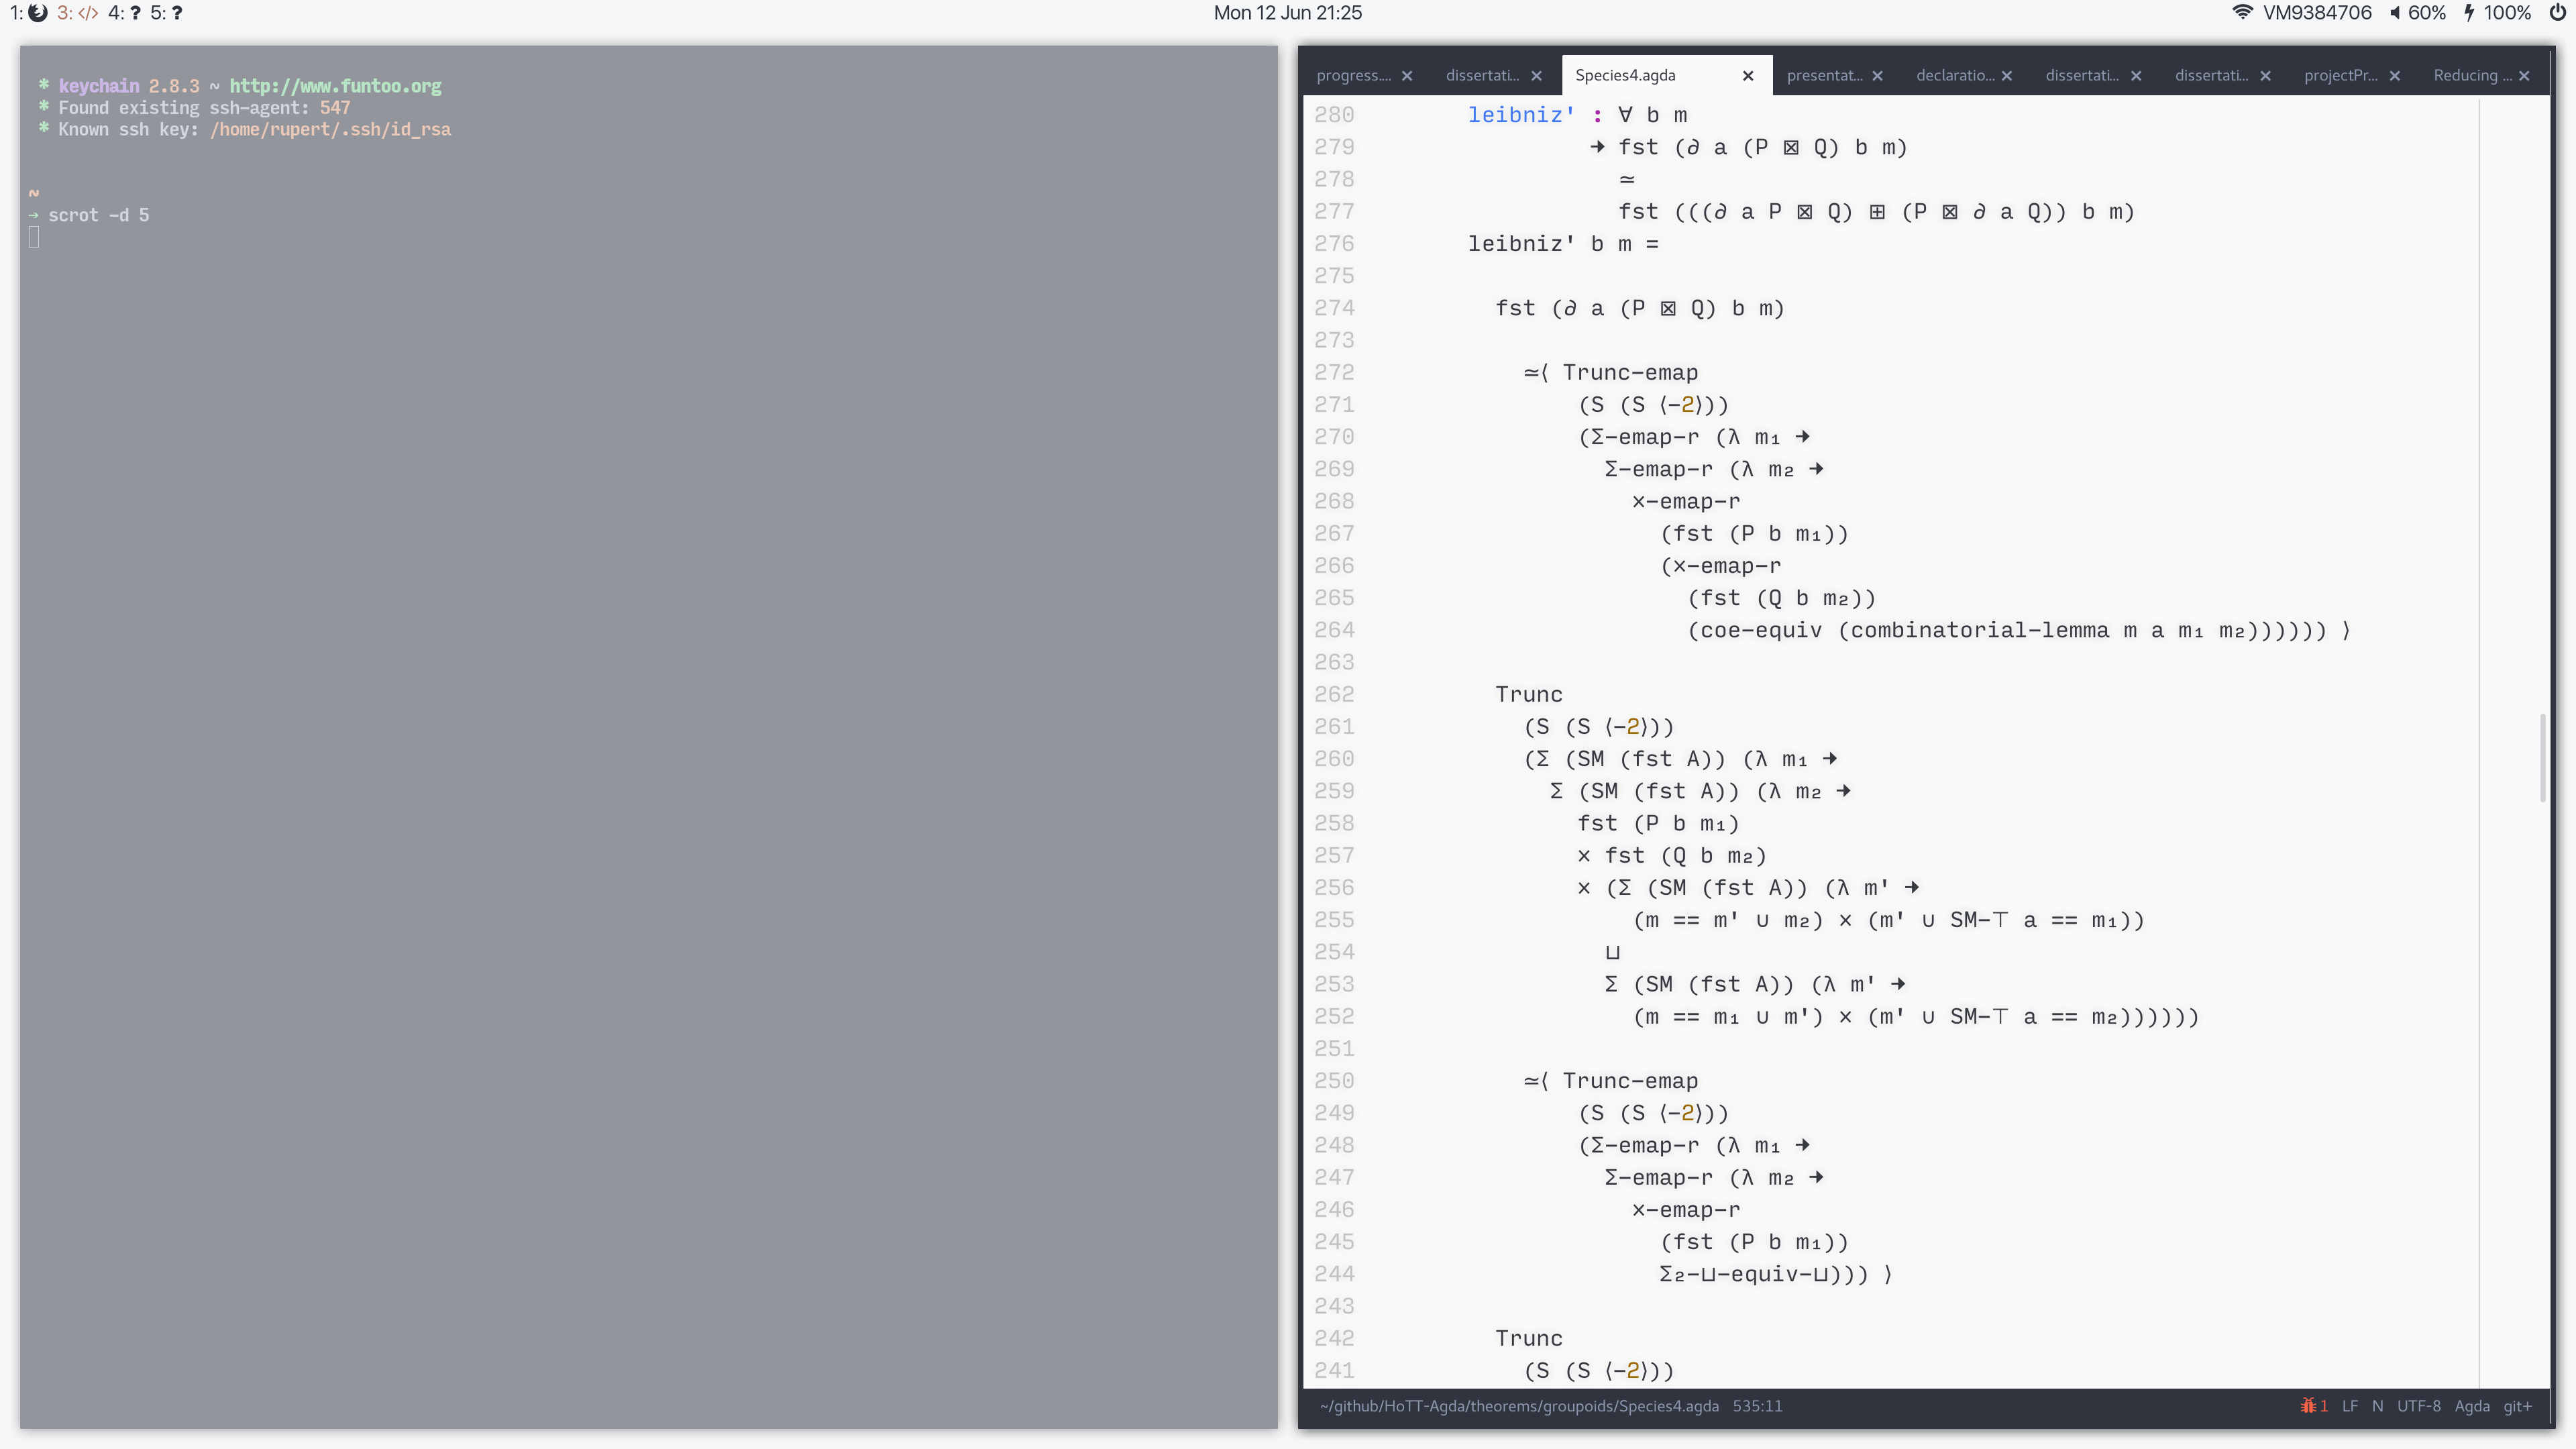
\includegraphics[scale=0.1,trim={75cm 7cm 6cm 5.3cm},clip]{leibniz1}
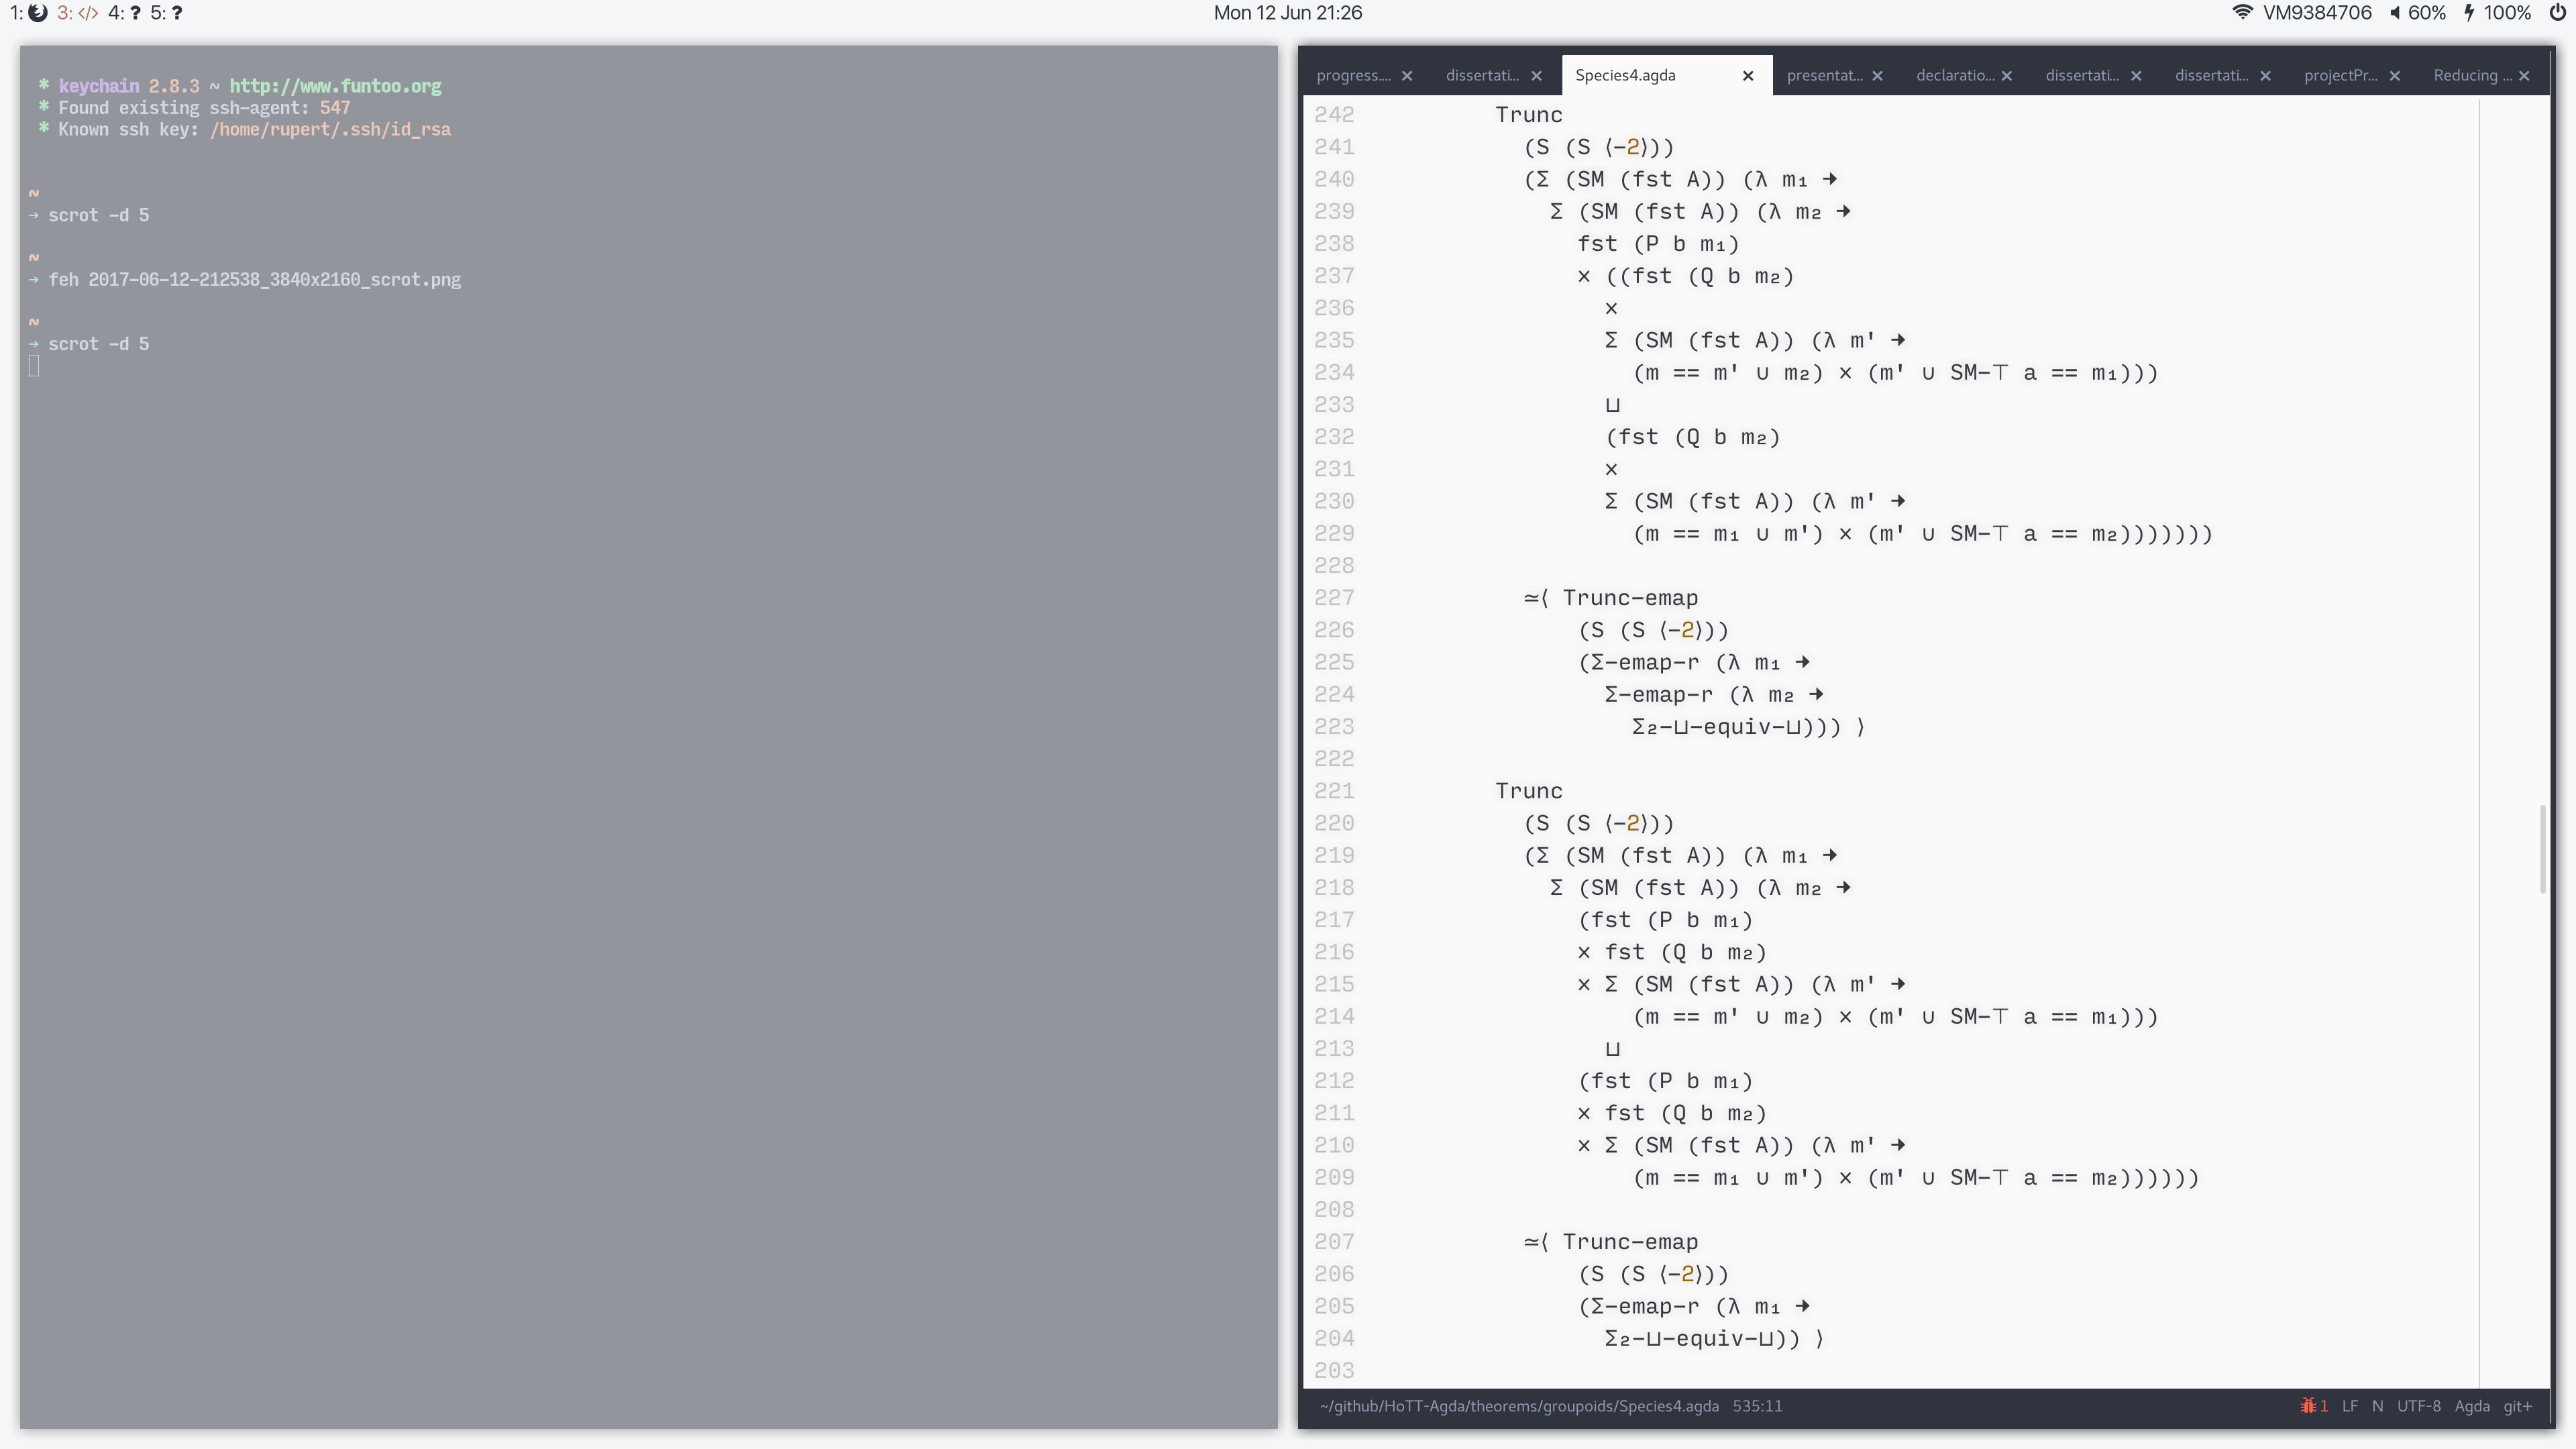
\includegraphics[scale=0.1,trim={75cm 7cm 6cm 5.3cm},clip]{leibniz2}
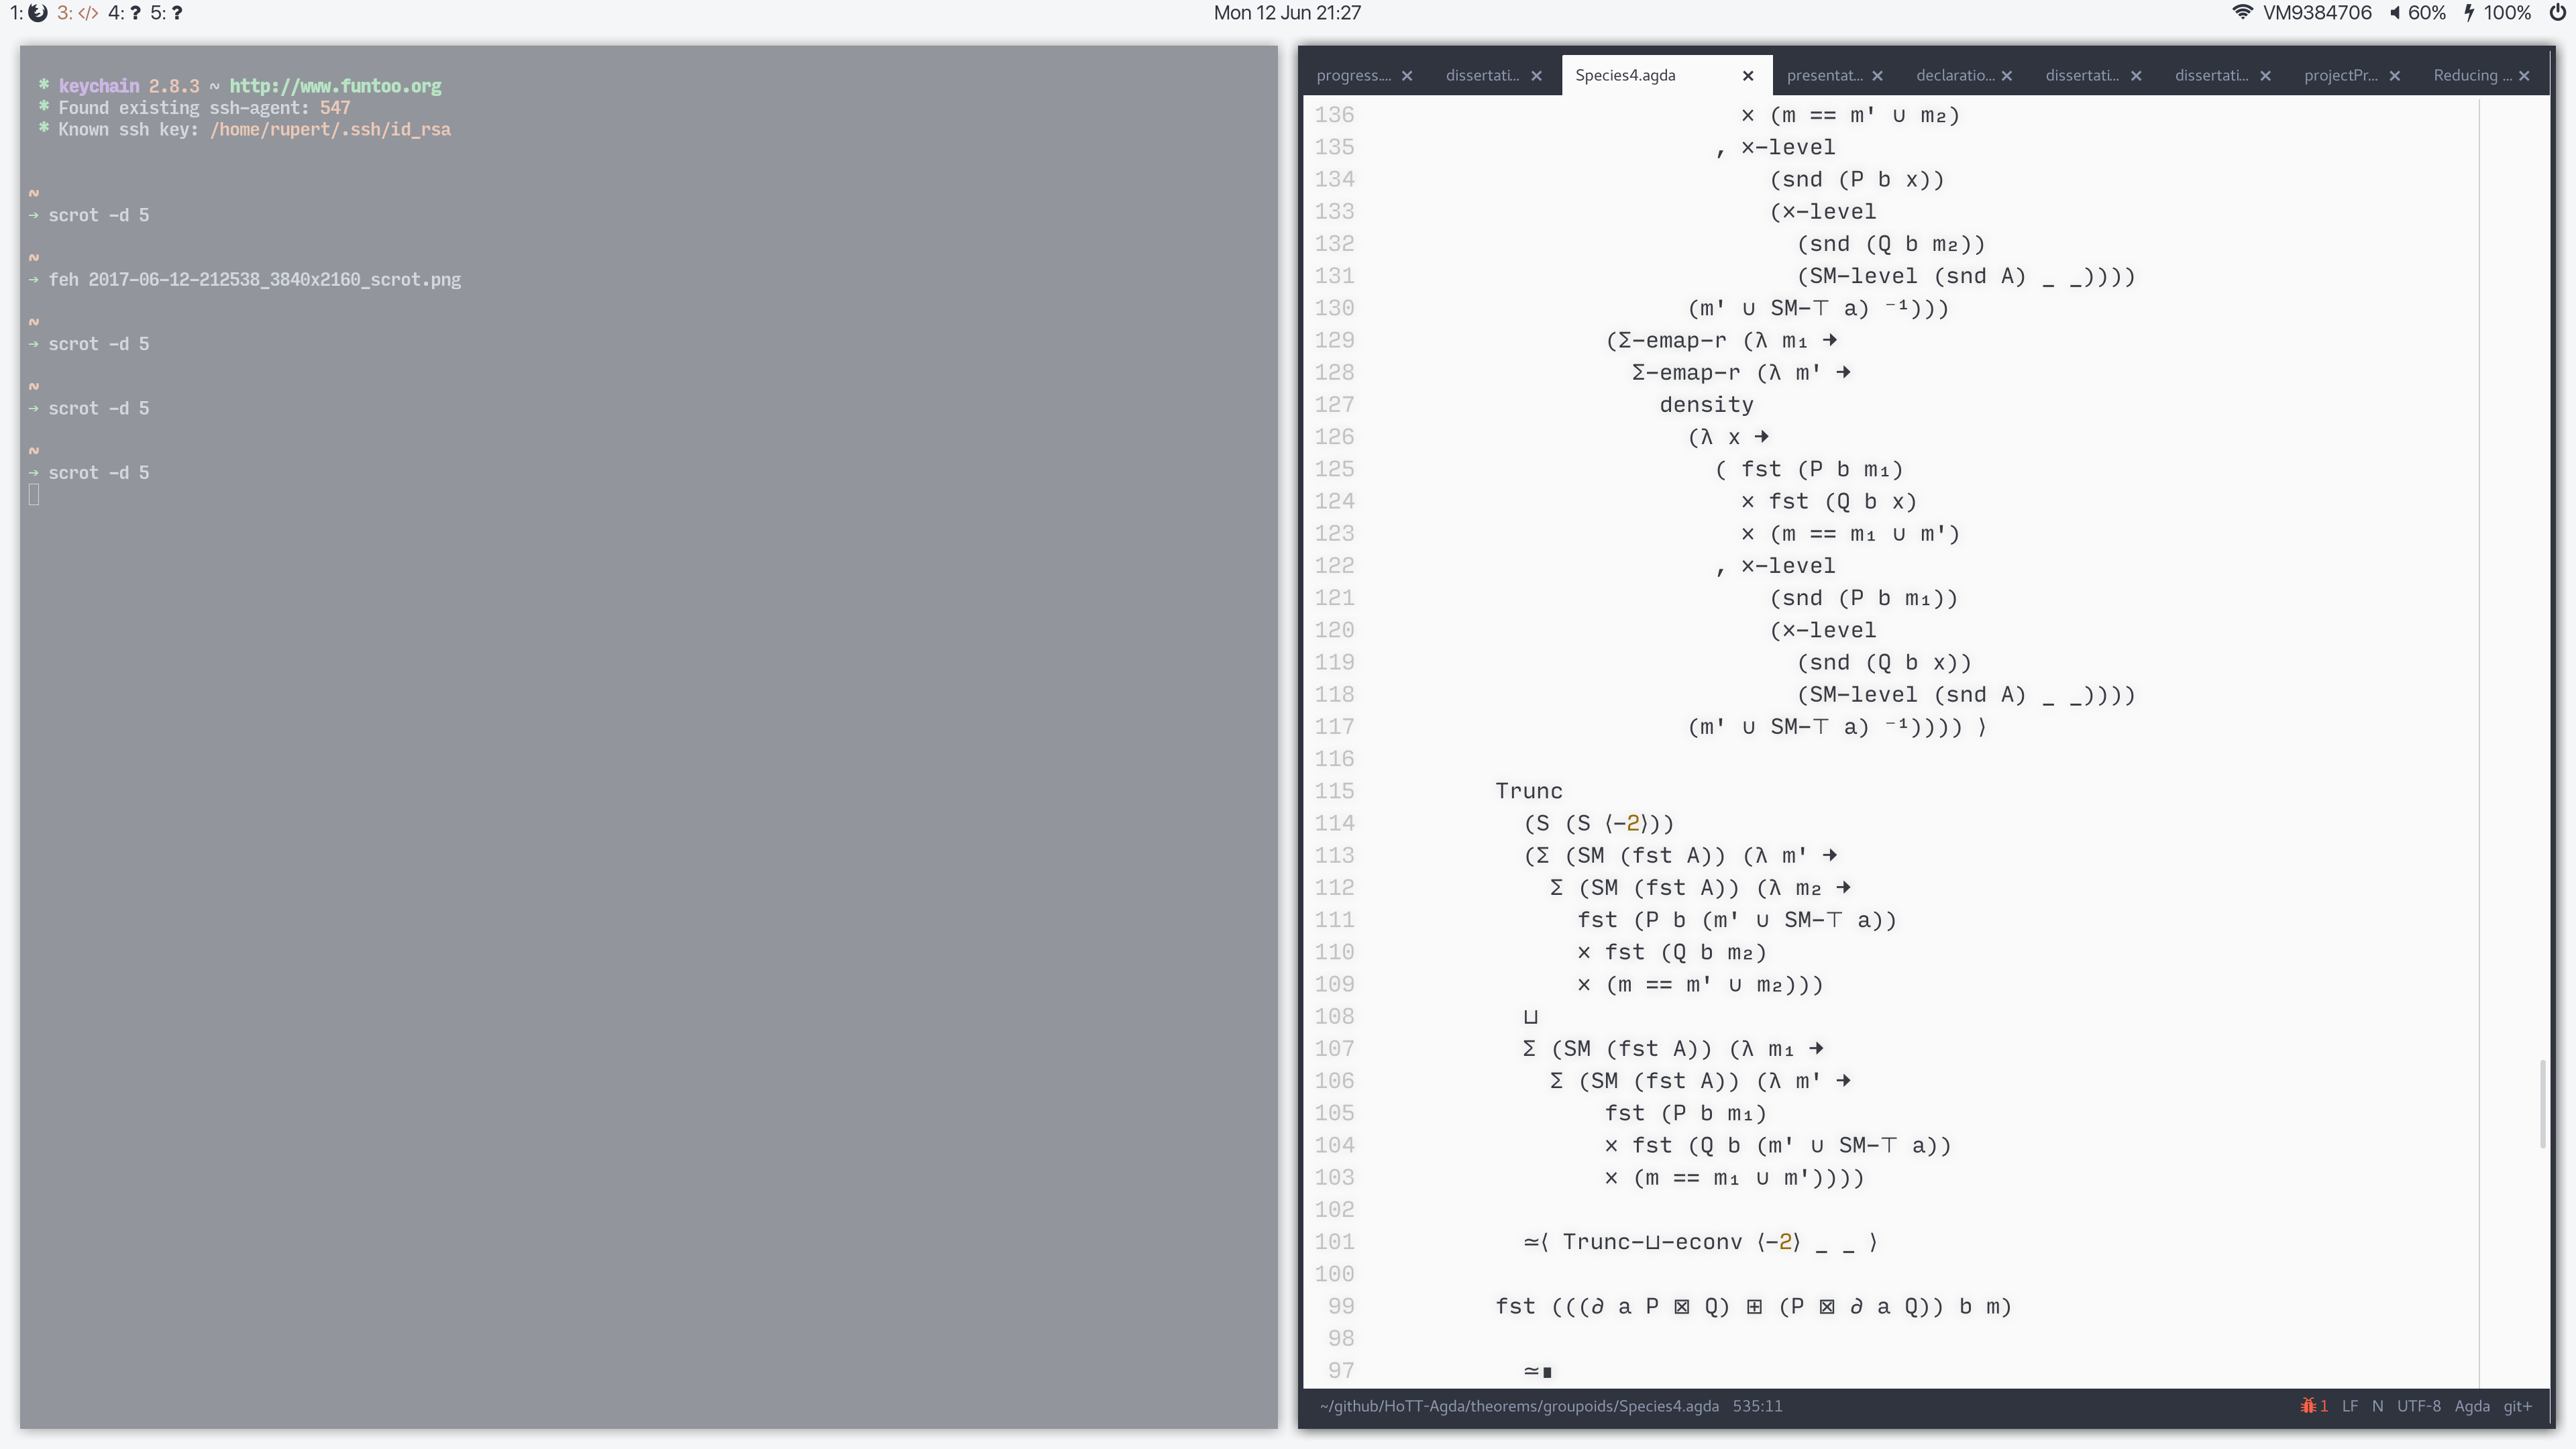
\includegraphics[scale=0.1,trim={75cm 3.2cm 6cm 9.1cm},clip]{leibniz4}
\end{center}

\clearpage

\thispagestyle{empty}

\begin{tikzpicture}[remember picture,overlay]
  \node [xshift=\paperwidth/2,yshift=-\paperheight/2] at (current page.north west) [rectangle,fill,inner sep=0pt,minimum width=\paperwidth,minimum height=\paperheight,top color=mybgcolor!64,bottom color=mybgcolor,text width=180mm,align=center,color=white] {\sffamily\huge Questions?};
\end{tikzpicture}

\end{document}
